% Optionen:
% Schriftgroesse: 12pt, 
% A4. Blocksatz
% *.tex als UTF8
% Keine Abschließenden Punkte (z.B. Abbildung 1.)
% Kein Abstand zwischen Kapiteln in Verzeichnissen
\documentclass[fontsize=12pt, paper=a4, utf8, numbers=noenddot, listof=nochaptergap, parskip=half]{scrreprt}

% deutsche Silbentrennung
\usepackage[ngerman]{babel}
\usepackage{blindtext}
		
% Umlaute unter UTF8 nutzen
\usepackage[utf8]{inputenc}

% Zeichenencoding
\usepackage[T1]{fontenc}
\usepackage{lmodern}

% Schriftart Arial
\usepackage{helvet}
\renewcommand{\familydefault}{\sfdefault}

% Kapitel auf neue Seite
\usepackage{titlesec}

% Zeilenumbruch in URL's
\usepackage[hyphens]{url}

% Verzeichnis formatieren
\usepackage[tocflat]{tocstyle}

% Abkürzungsverzeichnis
\usepackage{acronym}

% Beispiele und Beispielverzeichnis
\usepackage{listings}
\usepackage{minted}

% Literaturverzeichnis / zitieren
\usepackage[backend=bibtex,style=authoryear-icomp,sorting=nty, maxcitenames=2,natbib]{biblatex}
\addbibresource{Literatur.bib} 

% Kopf- und Fußzeilen flexibel gestalten
\usepackage[headsepline,footsepline]{scrpage2} 
\usepackage[bottom, hang]{footmisc}

% Referenzen
\usepackage[linkcolor=black, urlcolor=black, citecolor=black, colorlinks=true]{hyperref}

% Positionierung von Gleitobjekten
\usepackage{float}
\usepackage{wrapfig}
\usepackage[section]{placeins}

% Tabellen
\usepackage{array}

% Farben
\usepackage[table]{xcolor}
\usepackage{color}

% Grafiken
\usepackage{graphicx}

% Syntaxhighlighting
\usepackage{minted}
\usepackage{ragged2e}
\usepackage{etoolbox}
\usepackage{xpatch}

% Beschreibungsart Fett Darstellen und kleinere Schriftgröße
\usepackage[font=small,labelfont=bf,textfont=md]{caption}

% Anhänge
\usepackage{appendix}

% Checkboxen
\usepackage{wasysym}

% Einbinden von PDFs
\usepackage{pdfpages}

% kompakte Liste
\usepackage{mdwlist}

%~~~~~~~~~~~~~~~~~~~~~~~~~~~~~~~~~~~~~~~~~~~~~~~~~~~~~~~~~~~~~~~~~~~~~
%	Einstellungen
%~~~~~~~~~~~~~~~~~~~~~~~~~~~~~~~~~~~~~~~~~~~~~~~~~~~~~~~~~~~~~~~~~~~~~ 
% Bilderpfad festlegen
\graphicspath{{Images/}}

% Vermeiden einzelner Zeilen am Ende einer Seite oder oben auf einer neuen Seite
\clubpenalty10000
\widowpenalty10000

% Schriftgröße neu definieren
\setkomafont{chapter}{\fontsize{16bp}{18.8bp}\selectfont\bfseries}
\setkomafont{section}{\fontsize{14.5bp}{18.8bp}\selectfont\bfseries}
\setkomafont{subsection}{\fontsize{13bp}{18.8bp}\selectfont\bfseries}

% Abstände vor und nach der Kapitelüberschrift reduzieren
\RedeclareSectionCommands[
	beforeskip=0em,
	afterskip=0.1em
]{section,subsection,subsubsection}

% Zeilenabstand
\linespread{1.3}		         

% Kopf und Fußzeile
\pagestyle{scrheadings}
\renewcommand*\chapterpagestyle{scrheadings}
% Kopf- und Fußzeile nicht kursiv
\renewcommand*{\headfont}{\normalfont}
\renewcommand*{\footfont}{\normalfont}
% Kapitelübersicht automatisch in Kopfzeile setzen
\automark{chapter}
% Kapitelüberschrift mittig in Kopfzeile entfernen
\chead[]{}
% Kapitelüberschrift rechts in Kopfzeile
\renewcommand*{\chaptermarkformat}{} 
\ohead{\headmark}
% Seitenzahlen in Fußzeilenmitte entfernen	
\cfoot[]{}
% Seitenzahlen in Fußzeile rechts anordnen	
\ofoot{Seite \pagemark}
% Fußnoten werden nicht mehr ab zewiter Zeile eingerückt
\setlength{\footnotemargin}{0pt}

% Chapter nach oben Rücken
\renewcommand{\chapterheadstartvskip}{\vspace*{-1\topskip}}
\renewcommand{\chapterheadendvskip}{\vspace*{0.2\topskip}}

% Erstzeileneinzug auf 0pt
\setlength{\parindent}{0pt}

% Minted-Optionen für Syntaxhighlighting in Beispielen
\setminted{autogobble, breaklines, linenos, frame=single, baselinestretch=1, fontsize=\footnotesize}	

% Abbildungen, Tabellen und Fußnoten durchgehend nummerieren
% Durchgehend Numerieren
\counterwithout{figure}{chapter}
\counterwithout{table}{chapter}	
\counterwithout{footnote}{chapter}	

% Beispiele und -Verzeichnis umbennnen
\renewcommand{\listingscaption}{Beispiel}
\renewcommand{\listoflistingscaption}{Beispielverzeichnis}

% Inhaltsverzeichnis richtig einrücken
\RedeclareSectionCommand[tocindent=25mm,tocnumwidth=45mm]{subsection} 

% Abstand Überschrift Beispielverzeichnis anpassen
\addtocontents{lol}{\vskip 0.5em}  

% Abstand Literaturverzeichnis verringern
\setlength{\bibitemsep}{1em}

% Abkürzungsverzeichnis nicht fett darstellen
\renewcommand*\aclabelfont[1]{\acsfont{#1}}

% Bild-/Tabellen-/Beispielunterschrift Abstand verringern
\setlength{\belowcaptionskip}{-1.3em}

% Rote Boxen in Beispielen deaktivieren
\makeatletter
\AtBeginEnvironment{minted}{\dontdofcolorbox}
\def\dontdofcolorbox{\renewcommand\fcolorbox[4][]{##4}}
\xpatchcmd{\inputminted}{\minted@fvset}{\minted@fvset\dontdofcolorbox}{}{}
\makeatother

% Vorgabe der BA-Glauchau: Raender links 2.5cm, rechts 2.5cm, oben 2cm, unten 2cm
\usepackage[a4paper, left=2.5cm, right=2.5cm, top=2cm, bottom=2cm, bindingoffset=0mm, footskip=20pt, includeheadfoot]{geometry}


%Der folgende Code ersetzt im Literaturverzeichnis bei mehreren Werken desselben Autors den Strich durch den Autorennamen
% https://www.mrunix.de/forums/showthread.php?65454-biblatex-Literaturverzeichnis-gleiche-Autoren&s=a4c3d1baa8fc89f3422caf381c296fa6&p=298151&viewfull=1#post298151
\makeatletter	
\renewbibmacro*{author}{%
	\ifthenelse{\ifuseauthor\AND\NOT\ifnameundef{author}}
	{\ifthenelse{\iffieldequals{fullhash}{\bbx@lasthash}\AND
			\NOT\iffirstonpage}
		{\savefield{fullhash}{\bbx@lasthash}%
			\printnames{author}%
			\iffieldundef{authortype}
			{\setunit{\addspace}}
			{\setunit{\addcomma\space}}}
		{\savefield{fullhash}{\bbx@lasthash}%
			\printnames{author}%
			\iffieldundef{authortype}
			{\setunit{\addspace}}
			{\setunit{\addcomma\space}}}%
		\iffieldundef{authortype}
		{}
		{\usebibmacro{authorstrg}%
			\setunit{\addspace}}}%
	{\global\undef\bbx@lasthash
		\usebibmacro{labeltitle}%
		\setunit*{\addspace}}%
	}
\makeatother

% Anhangsverzeichnis am Ende (Lösung von hier: https://www.komascript.de/comment/3447#comment-3447)
\usepackage{filecontents}
\begin{filecontents}{appendixtoc.sty}
	%
	% appendixtoc.sty
	% Copyright (c) Markus Kohm, 2013-2017
	% See `appendixtocexample.tex' for license informations. Distribution without
	% `appendixtocexample.tex' is forbidden!
	% See <http://www.komascript.de/comment/3447#comment-3447> for more information.
	\ProvidesPackage{appendixtoc}[2017/05/03 unsupported LaTeX2e package]
	\RequirePackage{scrbase}[2013/12/19]% frühere Versionen unterstützen keine Sprachliste bei \providecaptionname
	\PackageWarningNoLine{appendixtoc}{This package uses obsolete `tocstyle'.\MessageBreak
		Recomment usage of alternative solution\MessageBreak
		https://komascript.de/node/2115}
	\RequirePackage{tocstyle}
	\usetocstyle{KOMAlike}
	% Die folgende Umgebung wird verwendet, um innerhalb der toc-Datei einzelne
	% Bereiche ein- und ausschalten zu können. In die toc-Datei wird die Umgebung
	% dabei jeweils als \begin{tocconditional}{BEREICH}...\end{tocconditional}
	% eingefügt.
	\newenvironment*{tocconditional}[1]{%
		\expandafter\ifx\csname if@toccond@#1\expandafter\endcsname
		\csname iftrue\endcsname
		\else
		\value{tocdepth}=-10000\relax
		\fi
		\typeout{tocdepth in `#1': \the\c@tocdepth}%
	}{%
	}
	
	% Gleich nach dem Öffnen der toc-Datei beginnen wir den Haupt-Bereich "main":
	\AtBeginDocument{%
		\addtocontents{toc}{\string\begin{tocconditional}{main}}
		}
		% Und der letzte Bereich endet am Ende der toc-Datei.
		\BeforeClosingMainAux{%
			\addtocontents{toc}{\string\end{tocconditional}}%
	}
	
	% Hier können nun neue Bereiche definiert (wie man das
	% macht zeigen wir gleich im Anschluss) ...
	\newcommand*{\newtocconditional}[2][false]{%
		\expandafter\newif\csname if@toccond@#2\endcsname
		\csname @toccond@#2#1\endcsname
	}
	% ... und ein- oder ausgeschaltet werden.
	% (Beispiele für die Verwendung von \settocconditional sind
	% weiter unten bei der Definition von \appendixtableofcontents
	% zu finden.)
	\newcommand*{\settocconditional}[2]{%
		\csname @toccond@#1#2\endcsname
	}
	
	% Neben dem (bereits aktivierten) Hauptbereich ...
	\newtocconditional[true]{main}
	% ... definieren wir noch einen (noch nicht aktivierten)
	% Bereich für den Anhang.
	\newtocconditional{appendix}
	
	% Mit dem Anhang geben wir einerseits das Anhangsverzeichnis aus,
	% andererseits beenden wir den aktuellen Bereich in der toc-Datei und beginnen
	% den neuen Bereich "appendix".
	% Für die Überschrift wird \tocbasic@listhead verwendet, damit das
	% Verzeichnis via \setuptoc{appendix}{…} (siehe Kapitel zu `tocbasic' in
	% der KOMA-Script-Anleitung) konfiguriert werden kann. Das passiert, bevor
	% der letzte Bereich geschlossen wird. Wenn wir es ganz sicher machen wollten,
	% müssten wir die auskommentierten Zeilen noch aktivieren. So verlassen wir
	% uns einfach darauf, dass vor dem appendix-Bereich der main-Bereich lag.
	\g@addto@macro\appendix{%
		%  \addtocontents{toc}{\string\end{tocconditional}^^J
		%    \string\begin{tocconditional}{main}}%
		\begingroup
		\@ifundefined{tocbasic@listhead}{% Falls \tocbasic@listhead (wird von
			% KOMA-Script-Klassen verwendet) nicht
			% definiert ist
			\@ifundefined{chapter}{% und falls \chapter nicht definiert ist,
				\section*{\listofappendixname}% \section* verwenden
			}{% aber falls \chapter definiert ist,
				\chapter*{\listofappendixname}% \chapter* verwenden
			}%
			% und noch die Kolumnentitel passend setzen.
			\@mkboth{\csname MakeMarkcase\endcsname{\listofappendixname}}%
			{\csname MakeMarkcase\endcsname{\listofappendixname}}%
		}{% Falls \tocbasic@listhead definiert ist,
			\def\@currext{appendix}% initialisieren
			\tocbasic@listhead{\listofappendixname}% und verwenden
		}%
		\endgroup
		\addtocontents{toc}{\string\end{tocconditional}^^J
		\string\begin{tocconditional}{appendix}}%
		\appendixtableofcontents
	}
	
	% Jetzt definieren wir das Anhangsverzeichnis selbst als Alias für die
	% toc-Datei. Dabei wird aber der Hauptbereich "main" deaktiviert und der
	% Anhangsbereich "appendix" aktiviert.
	\newcommand*{\appendixtableofcontents}{%
		\showtoc[{ %
			\aliastoc{\tocstyleTOC}{toc}%
			\settocconditional{main}{false}%
			\settocconditional{appendix}{true}%
		}]{toc}%
	}
	
	% Auch wenn man einen Anhang normalerweise nicht beenden kann, so ist es
	% ggf. erwünscht, dass Literaturverzeichnis, Index etc. zwar nach den Kapiteln
	% des Anhangs kommen, aber dem Hauptverzeichnis zugeordnet werden sollen. Also
	% benötigen wir eine Anweisung, um in der toc-Datei den aktuellen Bereich zu
	% beenden und wieder einen Hauptbereich einzuschalten:
	\newcommand*{\postappendix}{%
		\addtocontents{toc}{\string\end{tocconditional}^^J%
		\string\begin{tocconditional}{main}}%
	}
	
	% Den Namen definieren:
	\newcommand*{\listofappendixname}{Table of appendices}
	\AtBeginDocument{%
		\providecaptionname{american,australien,british,canadian,english,UKenglish,USenglish}\listofappendixname{Table of appendices}%
		\providecaptionname{german,ngerman,austrian,naustrian,swissgerman,nswissgerman}\listofappendixname{Anhangsverzeichnis}%
	}%
\end{filecontents}

\usepackage{appendixtoc}
% Wir wollen das Anhangsverzeichnis im Inhaltsverzeichnis, also sorgen wir
% dafür, dass das Paket tocbasic geladen ist (auch, wenn keine
% KOMA-Script-Klasse verwendet wird). Das muss unbedingt _vor_ dem Laden von
% appendixtoc passieren!
\usepackage{tocbasic}
\usepackage{appendixtoc}
\setuptoc{appendix}{totoc}% dank tocbasic geht das jetzt so einfach

%~~~~~~~~~~~~~~~~~~~~~~~~~~~~~~~~~~~~~~~~~~~~~~~~~~~~~~~~~~~~~~~~~~~~~
%	Begin Textteil - Befehle nur noch lokal Wirksam
%~~~~~~~~~~~~~~~~~~~~~~~~~~~~~~~~~~~~~~~~~~~~~~~~~~~~~~~~~~~~~~~~~~~~~ 
\begin{document}
	%======================================================================
%	Metadaten
%======================================================================
% Thema
\newcommand{\dcsubject}{Bachelorthesis} % evtl. Sperrvermerk und Eidesstattliche Erklärung anpassen
\newcommand{\dctitle}{Bachelorthesis Vorlage BA Glauchau LaTeX}
\newcommand{\dcdate}{20. August 2018}
\newcommand{\dckeywords}{hello,world}

% Autor
\newcommand{\dcauthorlastname}{Nachname}
\newcommand{\dcauthorfirstname}{Vorname}
\newcommand{\dcauthoremail}{e@mail.de}
\newcommand{\dcstreet}{Musterstraße, 17}
\newcommand{\dcplace}{12345, Musterstadt}

% BA
\newcommand{\dcuni}{Staatliche Studienakademie Glauchau}
\newcommand{\dccourse}{Technische Informatik}
\newcommand{\dcfield}{Daten- und Kommunikationstechnik}
\newcommand{\dcgroup}{Seminargr.}
\newcommand{\dcmatnr}{Matrikelnr.}

% Firma
\newcommand{\dccompany}{Mustermann GmbH GmbH}
\newcommand{\dccompanystr}{Musterstraße, 17}
\newcommand{\dccompanycity}{12345, Musterstadt}

% Betreuer
\newcommand{\refereecompany}{Dipl.-Ing. Moritz Mustermann}
\newcommand{\refereeuni}{Prof. Dr. Max Mustermann}

%%======================================================================
% Einstellungen des Hyperref-Paketes
\hypersetup
{
	pdftitle	= {\dctitle},
	pdfsubject	= {\dcsubject, \dcdate},
	pdfauthor	= {\dcauthorfirstname~\dcauthorlastname, \dcauthoremail},
	pdfkeywords	= {\dckeywords},
	pdfcreator	= {pdfTeX with Hyperref and Thumbpdf},
	pdfproducer	= {LaTeX, hyperref, thumbpdf}
}
%%====================================================================== 
	
	%======================================================================
	%	Titelseite
	%======================================================================
	%======================================================================
%	Titelseite 
%======================================================================
\begin{titlepage}
	\begin{bfseries}
		\begin{center}
			%Oberer Teil des Titelblattes
			\Huge{\dcsubject}\\[1cm]
			\Large{\dctitle}\\[2cm]
		\end{center}
	\end{bfseries}
			\begin{tabular}{p{4,3cm}l} % Tabulatoreinstellung
				\textbf{Vorgelegt am:}              & \dcdate\\[0.8cm]
				\textbf{Von:}                       & \textbf{\dcauthorfirstname~\dcauthorlastname}\\  
				                                    & \dcstreet\\
													& \dcplace\\[0.8cm]
				
				\textbf{Studiengang:} 				& \dccourse\\[0.8cm]
				
				\textbf{Studienrichtung:} 		    & \dcfield\\[0.8cm]
				
				\textbf{Seminargruppe:}             & \dcgroup\\[0.8cm]
				
				\textbf{Matrikelnummer:}            & \dcmatnr\\[0.8cm]
				
				\textbf{Praxispartner:}             & \dccompany\\
				                                    & \dccompanystr\\
				                                    & \dccompanycity\\[0.4cm]
				
		        \textbf{Gutachter:}                 & \refereecompany \\
                                                    & \dccompany \\\\
                                                    & \refereeuni\\
                                                    & \dcuni\\
			\end{tabular}
\end{titlepage}

	
	%======================================================================
	%	Themenblatt
	%======================================================================
	%\includepdf{Kapitel/Themenblatt}
	
	%======================================================================
	%	Sperrvermerk
	%======================================================================
	\newpage
\thispagestyle{empty}

%-----------------------------------
% Sperrvermerk
%-----------------------------------
\section*{Sperrvermerk}
Die vorliegende \dcsubject{} mit dem Titel: \\

\glqq\dctitle\grqq{} \\ \\ \\

beinhaltet interne und vertrauliche Informationen des Unternehmens: \\

\dccompany \\ \\ \\

Eine Einsicht in diese Bachelorarbeit ist nicht gestattet. Ausgenommen davon sind die betreuenden Dozenten sowie die befugten Mitglieder des Prüfungsausschusses. Eine Veröffentlichung und Vervielfältigung der \dcsubject{} – auch in Auszügen – ist nicht gestattet. \\

\par\medskip
\par\medskip


\_\_\_\_\_\_\_\_\_\_\_\_\_\_\_\_\_\_\_\_\_\_\_\_ \hspace{1.5cm} \_\_\_\_\_\_\_\_\_\_\_\_\_\_\_\_\_\_\_\_\_\_\_\_ \\
(Ort, Datum)\hspace{4.9cm}(Eigenhändige Unterschrift)

\newpage
	
	%======================================================================
	%	Verzeichnisse
	%======================================================================
	%======================================================================
%	Inahltsverzeichnis
%======================================================================
\cleardoubleemptypage
\pagenumbering{Roman}
\setcounter{page}{4}
\phantomsection
\addcontentsline{toc}{chapter}{Inhaltsverzeichnis}
\tableofcontents 

%======================================================================
%	Themenblatt
%======================================================================
\cleardoublepage
%\addcontentsline{toc}{section}{Themenblatt}

%======================================================================
%	Abbildungsverzeichnis
%======================================================================
\cleardoublepage
\phantomsection
\addcontentsline{toc}{chapter}{Abbildungsverzeichnis}
\listoffigures

%======================================================================
%	Tabellenverzeichnis
%======================================================================
\cleardoublepage
\phantomsection
\addcontentsline{toc}{chapter}{Tabellenverzeichnis}
\listoftables

%======================================================================
%	Quellcodeverzeichnis
%======================================================================
\cleardoublepage
\phantomsection
\addcontentsline{toc}{chapter}{Beispielverzeichnis}
\listoflistings

%======================================================================
%	Abkürzungsverzeichnis
%======================================================================
\cleardoublepage
\chapter*{Abkürzungsverzeichnis}
\addcontentsline{toc}{chapter}{Abkürzungsverzeichnis}
\manualmark
\markboth{Abkürzungsverzeichnis}{Abkürzungsverzeichnis}
\automark{chapter}

% Abstand richtet sich nach längster Abkürzung
% 10 Zeichen sollten in den meisten Fällen reichen
\begin{acronym}[0123456789]
	% Zeilenabstand verringern
	\setlength{\parskip}{0ex}
	\setlength{\itemsep}{1ex}
	
	\acro{HTTP}{Hypertext Transfer Protocol}
	\acro{HTTPS}{Hypertext Transfer Protocol Secure}
	\acro{URI}{Uniform Resource Identifier}
\end{acronym}

%%======================================================================
%%      Ende
%%======================================================================
\cleardoublepage
\pagenumbering{arabic}
	
	%======================================================================
	%	Inhalt
	%======================================================================	
	\sffamily
\chapter{Motivation und Aufgabenstellung}\label{cha:Motivation}

%%%%%%%%%%%%%%%%%%%%%%%%%%%%%%%%%%%%%%%%%%%%%%%%%%%%%%%%%%%%%%%%
% Motivation
%%%%%%%%%%%%%%%%%%%%%%%%%%%%%%%%%%%%%%%%%%%%%%%%%%%%%%%%%%%%%%%%
\section{Motivation}
\blindtext

%%%%%%%%%%%%%%%%%%%%%%%%%%%%%%%%%%%%%%%%%%%%%%%%%%%%%%%%%%%%%%%%
% Aufgabenstellung
%%%%%%%%%%%%%%%%%%%%%%%%%%%%%%%%%%%%%%%%%%%%%%%%%%%%%%%%%%%%%%%%
\section{Aufgabenstellung}
\blindtext
Mehr zu \acp{URI} kann der nachfolgenden Abbildung \ref{fig:uri} entnommen werden. Alles weitere Anhang \ref{anh:index}.

\begin{figure}[H]
	\centering
	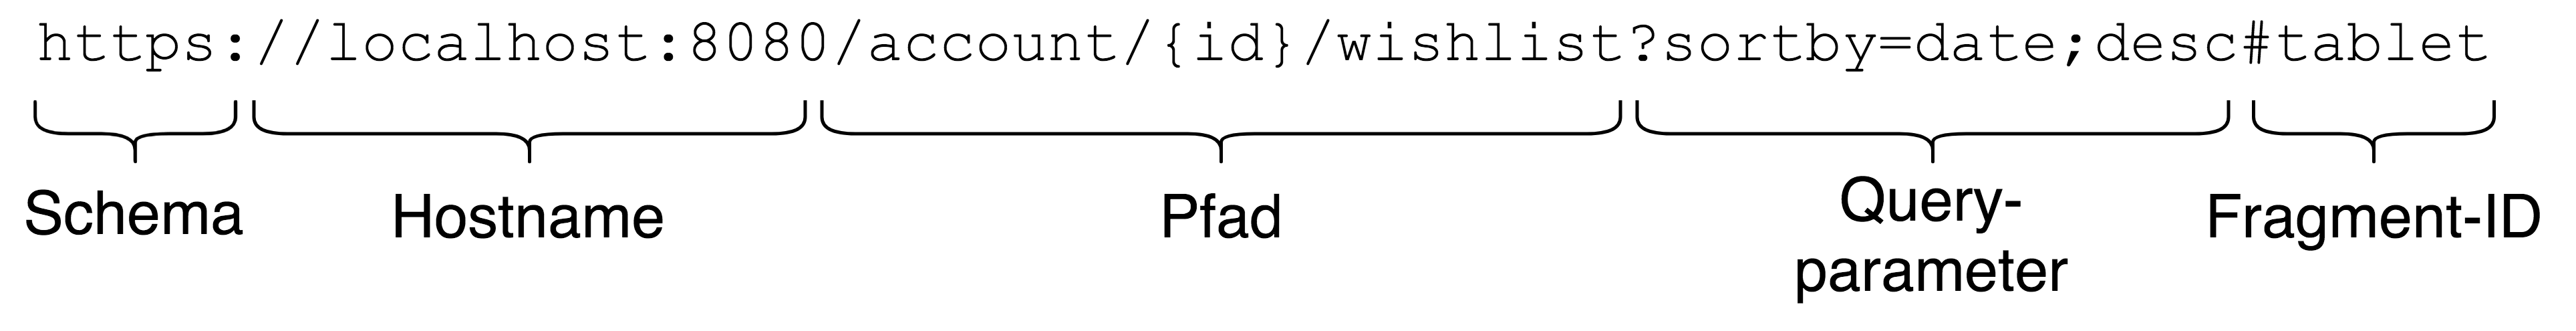
\includegraphics[scale=0.1]{uri-aufbau}
	\caption{Grundprinzip \acs{URI}}
	\label{fig:uri}
\end{figure}

\blindtext

	\sffamily
\chapter{Grundlagen}\label{cha:Grundlagen}

%%%%%%%%%%%%%%%%%%%%%%%%%%%%%%%%%%%%%%%%%%%%%%%%%%%%%%%%%%%%%%%%
% Webservice
%%%%%%%%%%%%%%%%%%%%%%%%%%%%%%%%%%%%%%%%%%%%%%%%%%%%%%%%%%%%%%%%
\section{Hello}
\blindtext

% Aufzählungen in kompakterer Darstellung
\begin{itemize*}
	\item eins,
	\item zwei,
	\item drei,
	\item usw.
\end{itemize*}

%%%%%%%%%%%%%%%%%%%%%%%%%%%%%%%%%%%%%%%%%%%%%%%%%%%%%%%%%%%%%%%%
% REST
%%%%%%%%%%%%%%%%%%%%%%%%%%%%%%%%%%%%%%%%%%%%%%%%%%%%%%%%%%%%%%%%
\section{World}
\blindtext\footnote{online: \Citealp{Fielding.2008} (16.07.2018)}
Mehr dazu in Tabelle \ref{tab:http_verben}.

\begin{table}[H]
	\centering
	\begin{tabular}{|c|>{\centering}m{1.3cm}|>{\centering}m{1.3cm}|m{9.5cm}|}
		\hline
		\multicolumn{1}{|>{\centering}c|}{\cellcolor{black!10}\textbf{Methode}} &
		\multicolumn{1}{>{\centering}m{1.3cm}|}{\cellcolor{black!10}\textbf{Si\-cher}} &
		\multicolumn{1}{>{\centering}m{1.3cm}|}{\cellcolor{black!10}\textbf{Idem\-potent}}  &
		\multicolumn{1}{>{\centering}m{9.5cm}|}{\cellcolor{black!10}\textbf{Beschreibung}} \\ \hline
		GET & \textbf{x} & \textbf{x} & Empfangen von Informationen, die durch eine \ac{URI} identifiziert werden und in Form einer Repräsentation vorliegen. \\ \hline
		HEAD & \textbf{x} & \textbf{x} & Liefern die Metadaten einer Ressource zurück. Müssen mit denen von GET übereinstimmen. \\ \hline
	\end{tabular}
	\caption{\acs{HTTP}-Standardmethoden}
	\label{tab:http_verben}
\end{table}
	\sffamily
\chapter{Analyse}\label{cha:Analyse}

%%%%%%%%%%%%%%%%%%%%%%%%%%%%%%%%%%%%%%%%%%%%%%%%%%%%%%%%%%%%%%%%
% Möglichkeiten zur Implementierung eines REST-Webservices
%%%%%%%%%%%%%%%%%%%%%%%%%%%%%%%%%%%%%%%%%%%%%%%%%%%%%%%%%%%%%%%%
\section{Implementierungsmöglichkeiten}
\subsection{A}
\blindtext

\subsection{B}
\blindtext

\begin{listing}[H]
	\inputminted{js}{Code/rest.js}
	\unskip
	\caption{REST-Service in JavaScript}
	\label{lst:rest_php}
\end{listing}
\unskip % wird bei Beispielen benötigt, da sonst der Abstand danach zu groß ist

%%%%%%%%%%%%%%%%%%%%%%%%%%%%%%%%%%%%%%%%%%%%%%%%%%%%%%%%%%%%%%%%
% Sicherheit eines REST-Webservice
%%%%%%%%%%%%%%%%%%%%%%%%%%%%%%%%%%%%%%%%%%%%%%%%%%%%%%%%%%%%%%%%
\section{Weiteres}
\blindtext
	\sffamily
\chapter{Implementierung}\label{cha:Implementierung}

\section{A}
\subsection{1}
\blindtext
\subsection{2}
\blindtext

\section{B}
\blindtext
Zitat mitten im Text (\Citealp[91]{Nguyen.2017}).
	\sffamily
\chapter{Fazit und Ausblick}\label{cha:Ausblick}
\blindtext
	
	%======================================================================
	%	Literaturverzeichnis
	%======================================================================
	% In Inhaltsverzeichnis und Kopfzeile aufnehmen
	\phantomsection
	\addcontentsline{toc}{chapter}{Literaturverzeichnis}
	\printbibliography[title=Literaturverzeichnis]
	
	%======================================================================
	%	Anhang
	%======================================================================
	%\manualmark
	\cleardoublepage
	%======================================================================	
%	Anhang
%======================================================================
\phantomsection
\appendix
\markboth{Anhangsverzeichnis}{Anhangsverzeichnis}

\clearpage
% Anänge mit Nummern, statt Buchstaben
\renewcommand*{\thechapter}{\arabic{chapter}}
% Fußzeile deaktivieren
\ofoot[]{}
% Kopfzeile neu beschriften
\ihead{\headmark}
\ohead{Anhang \thechapter}

\chapter{Einrichten des \acs{HTTP}- und \acs{HTTPS}-Servers (\textit{index.js})}
\label{anh:proto_index}
\inputminted{js}{Code/index.js}

	
	%======================================================================
	%	Eidesstattliche Erklaerung
	%======================================================================
	\clearpage
	\cleardoublepage
	%======================================================================
%	Eidesstattliche Erklärung
%======================================================================
\thispagestyle{empty}

\begin{center}
	\large Ehrenwörtliche Erklärung
\end{center}

\vspace{0.5cm}

\glqq Ich erkläre hiermit ehrenwörtlich\grqq{},

\vspace{1cm}

\begin{enumerate}
	\item[1.]  
	dass ich meine \dcsubject{} mit dem Thema:
	
	\glqq \dctitle \grqq{}
	
	ohne fremde Hilfe angefertigt habe,
	
	\item[2.] dass ich die Übernahme wörtlicher Zitate aus der Literatur sowie die Verwendung der Gedanken anderer Autoren an den entsprechenden Stellen innerhalb der Arbeit gekennzeichnet habe und
	
	\item[3.] dass ich diese \dcsubject{} bei keiner anderen Prüfung vorgelegt habe.	
\end{enumerate}

\vspace{1cm}

Ich bin mir bewusst, dass eine falsche Erklärung rechtliche Folgen haben wird.

\vspace{2cm}

\begin{tabular}{p{8cm}l}
	----------------------------------- &  ----------------------------------- \\
	(Ort, Datum) 					    &  (Unterschrift)  \\
\end{tabular}
\end{document}